\section{Experiments}

The objective of this experiment is to classify images into three hair types. To achieve this, we tested different hyperparameters, explored various preprocessing tecniques and experimented in creating the optimal CNN architecture. The primary goals in this experiment were to optimize evaluation metrics and minimize overfitting, ensuring robust model performance.

\subsection{Adjustment of Image Size and Batch Size}

The initial image size was set to $64 \times 64$ pixels. While this smaller dimension allowed us to train the model faster, it compromised the quality of the training images, potentially eliminating important information for accurate classification. Conversely, increasing the image size to $512 \times 512$ pixels significantly increased the training time to almost 30 minutes, which was impractical for our computational resources. Our experiments was conducted on a laptop with specifications of a GTX 1660Ti graphics card, a Ryzen 7 4800H processor, and 32GB of RAM.

\cite{impact_image_resolution} discussed in their paper that the performance of the classification model is dependent upon the resolution of images, but it is important to consider the trade-off between image size and the time needed for training the model. Considering these factors, we opted to use an image size of $256 \times 256$ pixels. This resolution provides an optimal balance between image quality and manageable training times. 

\begin{figure}[H]
    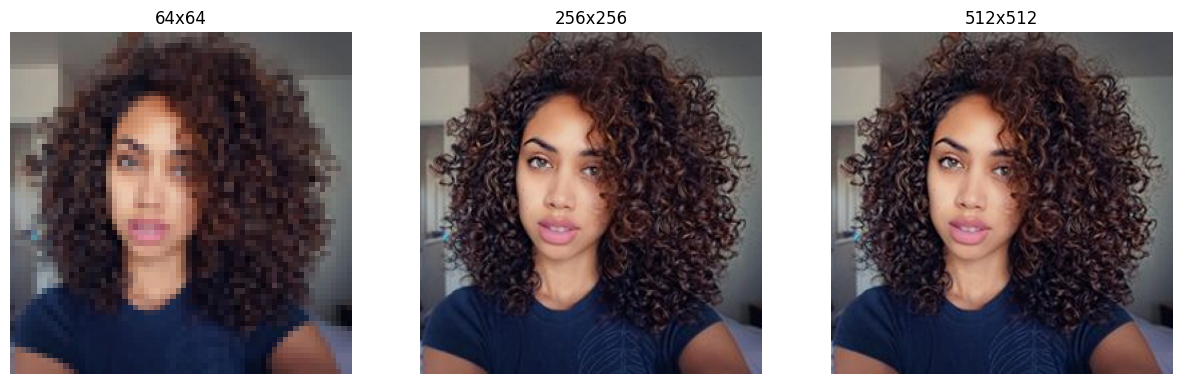
\includegraphics[width=\linewidth]{figures/image_sizes.png}
    \caption{Different Image Resolution}
    \label{fig:image_sizes}
  \end{figure}

Regarding the batch size, we experimented with sizes that are divisible by our image size, such as 32, 64, and 128. The batch size of 64 was chosen as it offers an efficient balance between minimizing the memory usage during training while providing a reliable estimate of the gradient. 

\subsection{Preprocessing}

During the experimental phase, we utilized two preprocessing techniques in machine learning for image classification: Sobel Edge Detection and Data Augmentation. These methods were chosen based on their potential to improve model accuracy and minimize overfitting.

The models were evaluated under four different preprocessing scenarios to assess their impact:

\begin{itemize}
    \item No preprocessing
    \item Sobel Edge Detection only
    \item Data Augmentation only
    \item Both Sobel Edge Detection and Data Augmentation
\end{itemize}

\begin{table}[H]
  \centering
  \caption{Comparative Results of Different Preprocessing Techniques: none, Sobel Edge Detection only, data augmentation only, and both}
  \label{tab:preprocessing_results}
  \begin{tabularx}{\linewidth}{>{\centering}X|>{\centering}X>{\centering}X>{\centering}X>{\centering\arraybackslash}X}
  \toprule
  & T Acc & Val Acc & T Loss & V Loss \\
  \midrule
  None & 0.639200 & 0.543100 & 0.771500 & 0.998300 \\
  \midrule
  Sobel only & 0.614500 & 0.586700 & 0.839800 & 1.010100 \\
  \midrule
  Data Aug only & 0.431100 & 0.543100 & 1.088000 & 0.983300 \\
  \midrule
  Both & 0.404100 & 0.411200 & 1.173300 & 1.111400 \\
  \bottomrule
  \end{tabularx}
\end{table}

The results from each scenario are shown in the Table \ref{tab:preprocessing_results}. Alongside these numerical results, we also provided plots of accuracy and loss to better illustrate the models' tendencies to overfit or underfit.

\begin{figure}[H]
  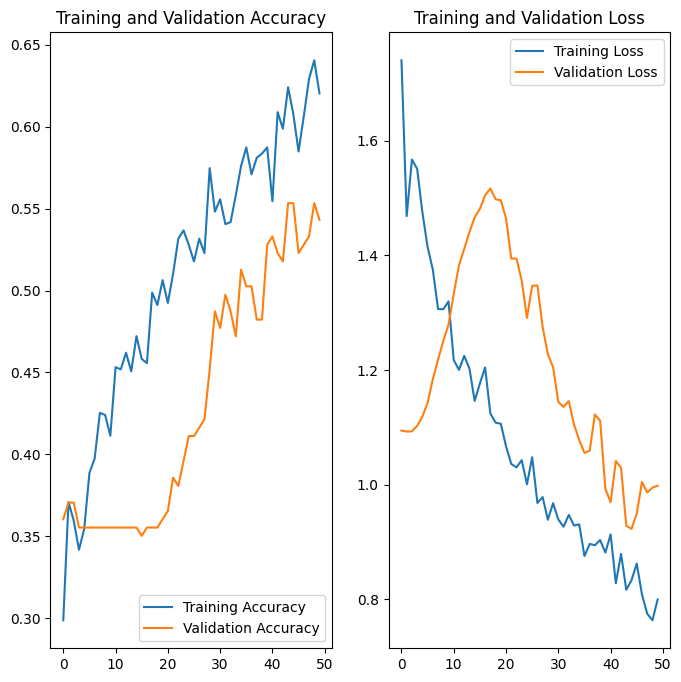
\includegraphics[width=\linewidth]{figures/without_preprocessing.png}
  \caption{No Preprocessing}
  \label{fig:no_preprocessing_plots}
\end{figure}

\begin{figure}[H]
  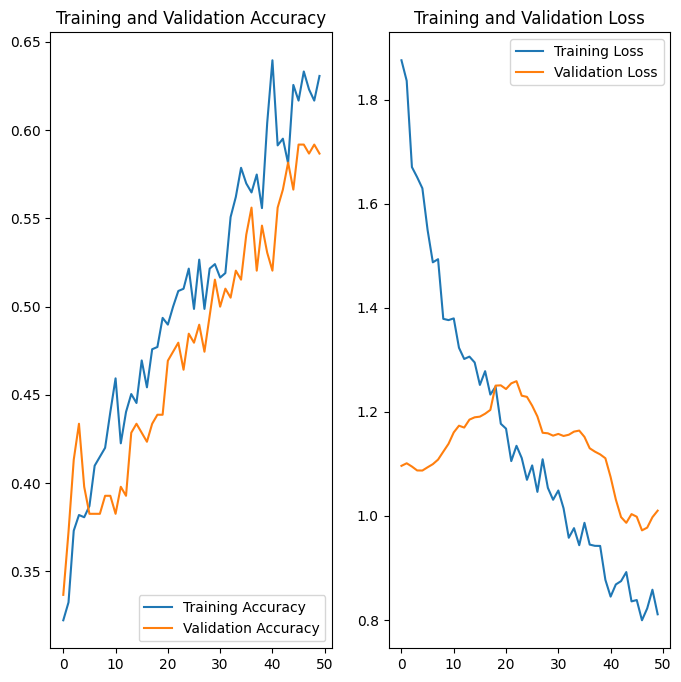
\includegraphics[width=\linewidth]{figures/training_validation_results.png}
  \caption{Sobel Edge Detection only}
  \label{fig:sobel_edge_plots}
\end{figure}

\begin{figure}[H]
  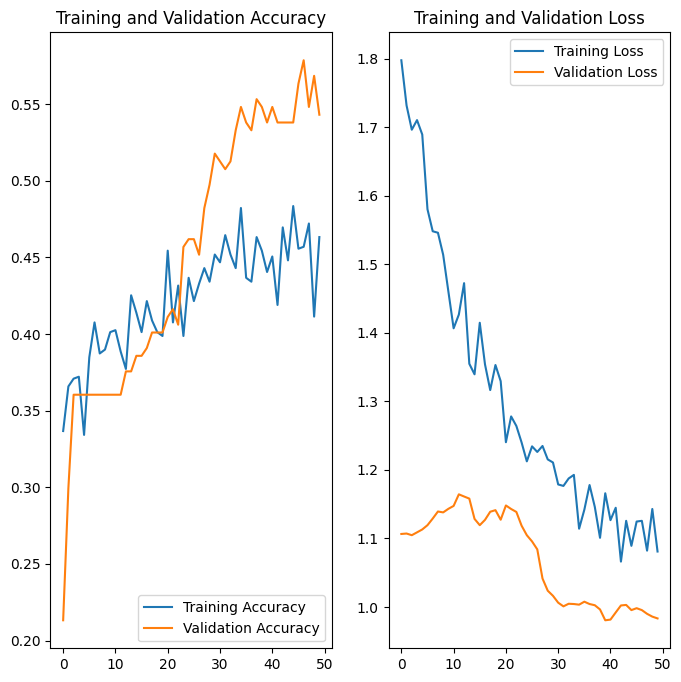
\includegraphics[width=\linewidth]{figures/with_data_aug.png}
  \caption{Data Augmentation only}
  \label{fig:data_aug_plots}
\end{figure}

\begin{figure}[H]
  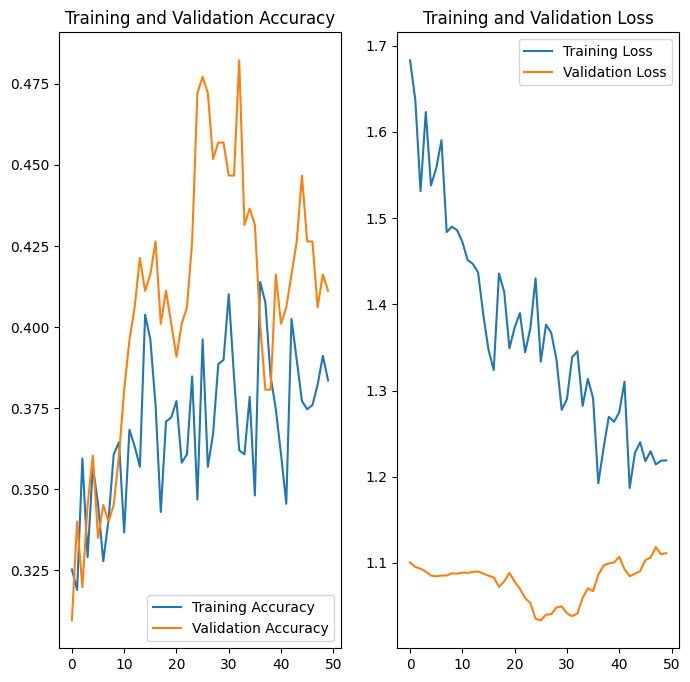
\includegraphics[width=\linewidth]{figures/with_data_aug_and_sobel_edge.png}
  \caption{Both Sobel Edge Detection and Data Augmentation}
  \label{fig:sobel_edge_and_data_aug_plots}
\end{figure}

The use of sobel edge detection helped improve object detection and segmentation, notably enhancing hair boundary delineation in the images, as seen in Figure \ref{fig:sobel_edge_plots}. Given that our dataset consists of only 987 valid images, data augmentation was important in addressing the limited data situation. Despite its benefits, the best model performance was obseved with Sobel Edge Detection only, leading us to exlude data augmentation in next phases.

\subsection{Modeling}

In developing an effective CNN for our classification task, our goal was to strike a balance between a sufficient number of convolutional layers to capture relevant features and maintaining the model's complexity, which is good for generalizability. 

\subsubsection{Create a Simple Model}

Our initial model was designed to be simple, serving as our starting point for exploration and providing insights about the straightforward application of convolutional layers. It is structured as follows:

\begin{enumerate}
  \item Convolutional layers with filter sizes of \(16\), \(8\), and \(4\), and corresponding filter counts of \(8\), \(16\), and \(32\), each followed by ReLU activation.
  \item A Global Average Pooling layer for dimensionality reduction.
  \item A dense layer with \(32\) units for pattern learning.
  \item A softmax output layer with \(3\) units for class prediction.
\end{enumerate}

\begin{figure}[H]
  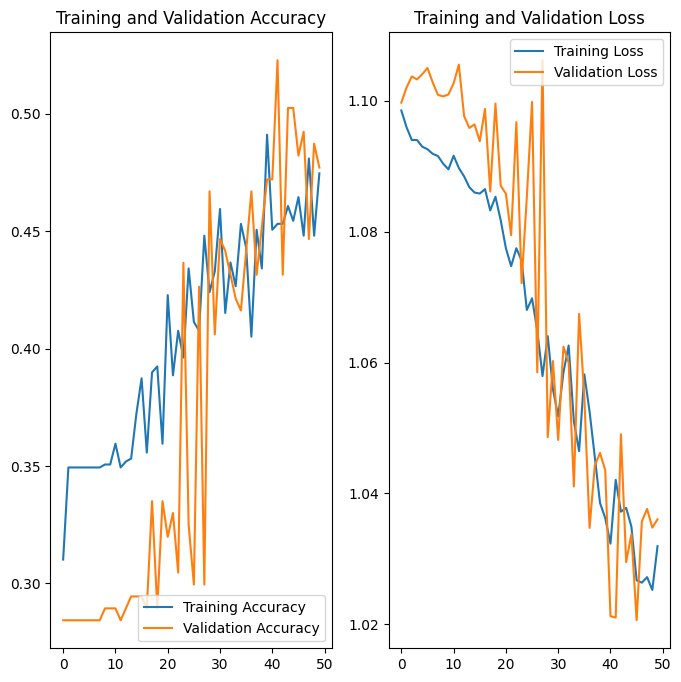
\includegraphics[width=\linewidth]{figures/simple_model.png}
  \caption{Accuracy and Loss Plots of the Simple Model}
  \label{fig:simple_model}
\end{figure}

After training the simple CNN model, we observed in Figure \ref{fig:simple_model} that the accuracy are fluctuating, which could suggest the need for normalization and additional layers to prevent it in overfitting. Both the training and validation losses decrease over time, which indicates that the model is learning. However, there is still a tendency to underfit, suggesting that the model is still too simple. Thus, this needs more experimentation with additional layers to capture more complex patterns.

\subsubsection{Add More Layers}

With insights gained from the simple model, we advanced our experimentation by increasing the model's complexity. We hypothesized that a greater number of convolutional layers would enable the capture of more patterns, which could be beneficial for the classification task, given the differences between hair types.

Following the initial experiment we made, we gained insights that helped us create a better model to meet our objectives. We hypothesized that adding more convolutional layers would help the model capture more important patterns. Increasing its complexity could be beneficial for our classification task, given that the dataset has multiple classes. The new model is structured as follows:

\begin{enumerate}
  \item Convolutional blocks with \(3 \times 3\) filters, ReLU activations, and \(2 \times 2\) max pooling, increasing filter counts in a doubling pattern.
  \item Global Average Pooling layer, a fully connected dense layer, and a softmax output layer, similar with the simple model architecture.
\end{enumerate}

\begin{figure}[H]
  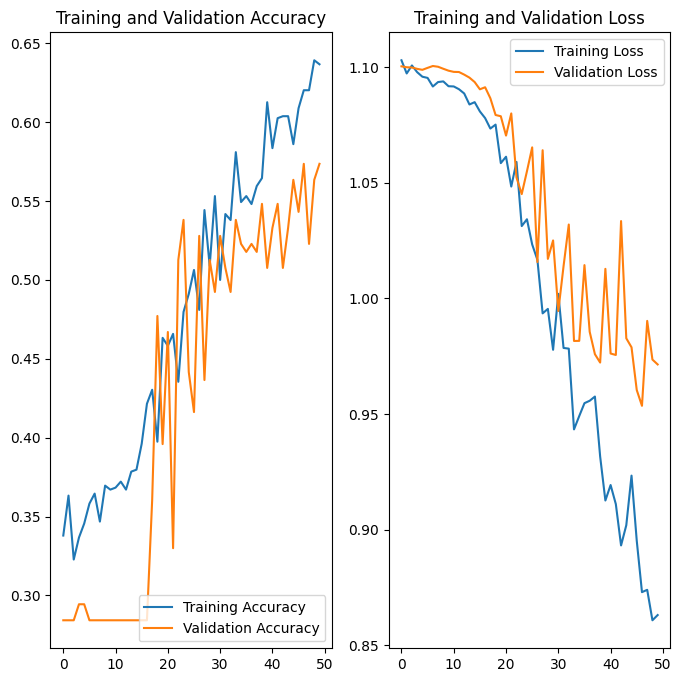
\includegraphics[width=\linewidth]{figures/many_layers.png}
  \caption{Accuracy and Loss Plots of the More Convolutional Layers Model}
  \label{fig:many_layers}
\end{figure}

This model's training and validation metrics, as depicted in Figure \ref{fig:many_layers}, demonstrate a noticeable improvement in performance compared to the simple model. The training accuracy shows a steady increase with less fluctuation, while the validation accuracy stabilizes. Similarly, the training and validation loss curves show a more consistent decrease, suggesting a better fit to the data.

It can be seen that there is a slight divergence of training and validation loss towards the later epochs, which may suggest the start of overfitting. We hypothesize that this could be resolved by adding dropout layers or introducing \texttt{BatchNormalization}.

\subsubsection{Flatten and Dropout}

We also wanted to evaluate the effects of using a \texttt{Flatten} layer in place of \texttt{GlobalAveragePooling2D}. This help us to retain all the information from the feature map. However, we are aware that using this can potentially cause overfitting, which is why we also implemented dropout layers. This modified architecture with \texttt{Flatten} and dropout layers is structured as follows:

\begin{enumerate}
  \item A series of convolutional layers with ReLU activations and batch normalization.
  \item Dropout layers set at 0.25 following the first two convolutional layers.
  \item A Flatten layer for vectorizing the feature maps before classification.
  \item An expanded dense layer with 512 units for complex pattern learning.
  \item A subsequent dropout layer with a rate of 0.5 following the dense layer.
  \item A softmax output layer for probabilistic class predictions.
\end{enumerate}

\begin{figure}[H]
  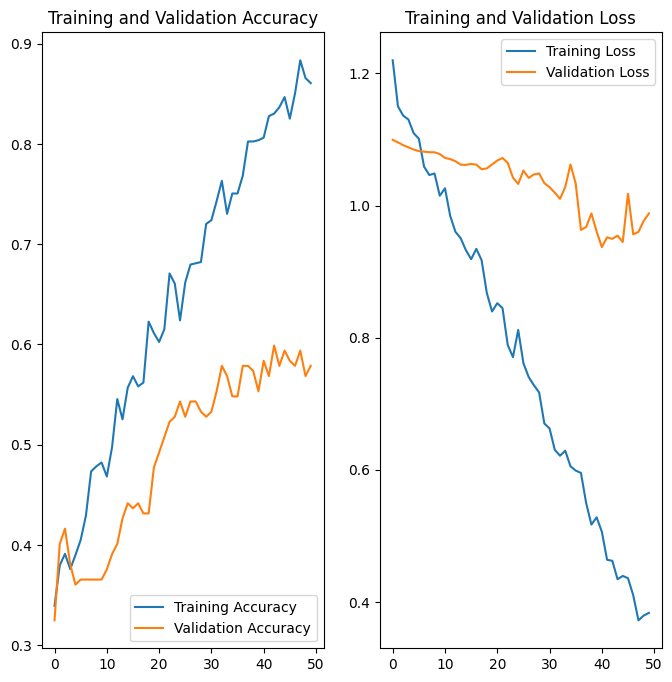
\includegraphics[width=\linewidth]{figures/flatten_model.png}
  \caption{Training and Validation Accuracy and Loss with Flatten and Dropout Layers}
  \label{fig:flatten_model}
\end{figure}

In the training and validation plots (Figure \ref{fig:flatten_model}), we can see that the training accuracy significantly increased, approaching a high of nearly 0.90. However, the model still exhibits signs of overfitting, despite the application of dropout layers to mitigate this issue. This is evidenced by the widening gap between the training and validation plots.

\subsubsection{Leaky ReLU}

In an effort to further refine our model, we implemented \texttt{Leaky ReLU} activation in our convolutional layers. \texttt{Leaky ReLU} is designed to overcome the limitations of the \texttt{ReLU function}. The modified architecture with Leaky ReLU is structured as follows:

\begin{enumerate}
  \item Convolutional layers with Leaky ReLU activations set with an alpha of 0.1.
  \item Batch normalization layers following each convolutional operation.
  \item Dropout layers after sets of convolutional layers with a 0.25 rate.
  \item A sequence of a Global Average Pooling layer followed by a Flatten layer.
  \item A dense layer with a following dropout stage, leading to a softmax output layer.
\end{enumerate}

\begin{figure}[H]
  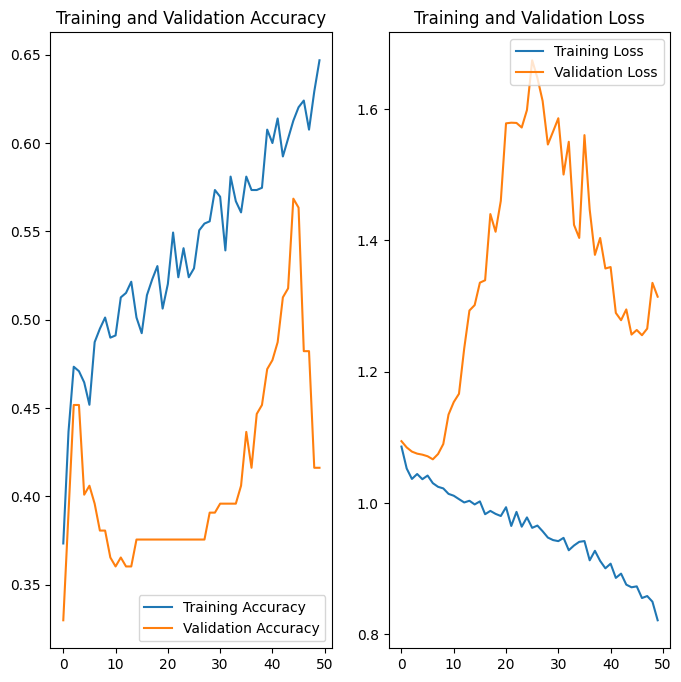
\includegraphics[width=\linewidth]{figures/leaky_relu.png}
  \caption{Training and Validation Accuracy and Loss with Leaky ReLU}
  \label{fig:leaky_relu}
\end{figure}

As illustrated in the training and validation plots (Figure \ref{fig:leaky_relu}), there is a wide gap between the training and validation curves. This model performed worse compared to the other models we developed earlier.

\subsubsection{Final Model}

Leveraging the insights gained from our initial explorations, we have developed a final model aimed at surpassing the performance of our previous experiments. This final model represents a combination  of techniques and layer structures that we hypothesize to be optimal for maximizin classification accuracy while avoiding overfitting. The final architecture is structured as follows:

\begin{enumerate}
  \item A $16 \times 16$ filter convolutional layer with ReLU activation and batch normalization.
  \item Additional convolutional layers with increased filter counts and reduced kernel sizes, each paired with ReLU activation, batch normalization, and max pooling.
  \item Dropout layers implemented after pooling layers with a 0.25 dropout rate for the first two sets of convolutional layers.
  \item A sequence of a Global Average Pooling layer followed directly by a Flatten layer.
  \item A dense layer with 32 units, accompanied by a 0.5 dropout rate, culminating in a 3-unit softmax output layer.
\end{enumerate}

The final model's performance, as showin in Figure \ref{fig:sobel_edge_plots}, reflects the enhancements made during our experimentation phase. The accuracy plot reveals the most favorable outcomes compared to the prior models. It demonstrated the effectiveness of the modified CNN structure catered to our dataset. The integration of significant elements from prvious models, combined with additional fine-tuning, gave us an outcome that displays minimial overfitting compared to earlier versions. With this advanced model, we expected better results compared to others, which will be discussed in the next chapter. 

\subsubsection{Optimizer Configuration}

In optimizing our CNN model, we chose the Adam optimizer for its adaptability and efficiency with sparse gradients. We initially set the learning rate of $1 \times 10^{-3}$ to test our experiments, but observed a tendency to overfit. According to Vishwakarma (2024) \cite{adam_optimizer}, the level recommended for balancing fast convergence and training stability is \(1 \times 10^{-4}\), which is why we used it throughout the recorded experiments. Additionally, the use of \texttt{categorical\_crossentropy} is suitable for our model because we have a multi-class dataset.

\subsection{U-Net model}

We have also tried to dabble with other architectures that have been proposed in the past for Convolutional Neural Networks. One architectur that we implemented is the U-Net architecture by \cite{ronneberger_u-net:_2015}. By following their simple architecture, without using any dropout layers, using different activation functions, etc. this model is actually able to achieve a good performance. As seen in figure \ref{unet}, the model is capable in its base form.

\begin{figure}[H]
  \centering
  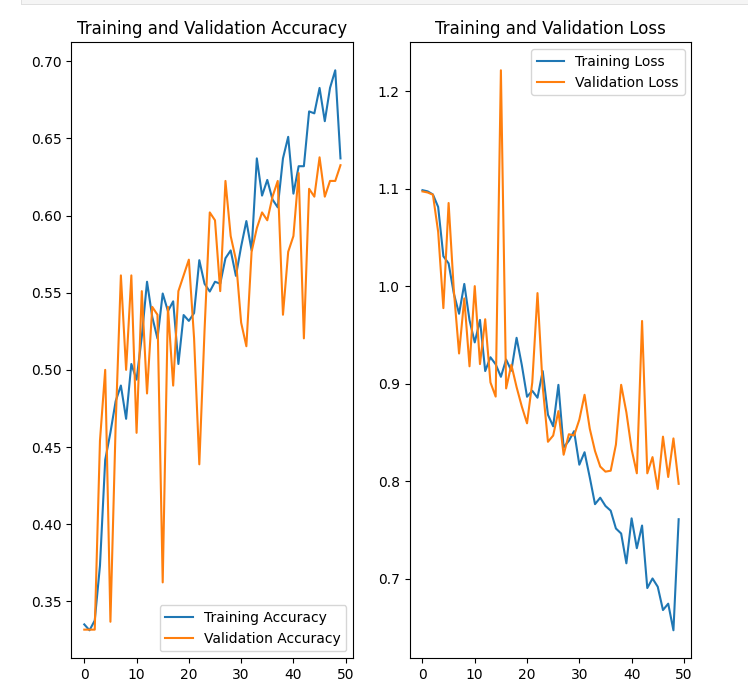
\includegraphics[width=0.8\linewidth]{figures/u_net.png}
  \caption{U-Net Performance History}
  \label{unet}
\end{figure}
